% Options for packages loaded elsewhere
\PassOptionsToPackage{unicode}{hyperref}
\PassOptionsToPackage{hyphens}{url}
%


\PassOptionsToPackage{table}{xcolor}

\documentclass[
  10pt,
  letterpaper,
]{article}

\usepackage{amsmath,amssymb}
\usepackage{iftex}
\ifPDFTeX
  \usepackage[T1]{fontenc}
  \usepackage[utf8]{inputenc}
  \usepackage{textcomp} % provide euro and other symbols
\else % if luatex or xetex
  \usepackage{unicode-math}
  \defaultfontfeatures{Scale=MatchLowercase}
  \defaultfontfeatures[\rmfamily]{Ligatures=TeX,Scale=1}
\fi
\usepackage{lmodern}
\ifPDFTeX\else  
    % xetex/luatex font selection
\fi
% Use upquote if available, for straight quotes in verbatim environments
\IfFileExists{upquote.sty}{\usepackage{upquote}}{}
\IfFileExists{microtype.sty}{% use microtype if available
  \usepackage[]{microtype}
  \UseMicrotypeSet[protrusion]{basicmath} % disable protrusion for tt fonts
}{}
\makeatletter
\@ifundefined{KOMAClassName}{% if non-KOMA class
  \IfFileExists{parskip.sty}{%
    \usepackage{parskip}
  }{% else
    \setlength{\parindent}{0pt}
    \setlength{\parskip}{6pt plus 2pt minus 1pt}}
}{% if KOMA class
  \KOMAoptions{parskip=half}}
\makeatother
\usepackage{xcolor}
\usepackage[top=0.85in,left=2.75in,footskip=0.75in]{geometry}
\setlength{\emergencystretch}{3em} % prevent overfull lines
\setcounter{secnumdepth}{-\maxdimen} % remove section numbering


\providecommand{\tightlist}{%
  \setlength{\itemsep}{0pt}\setlength{\parskip}{0pt}}\usepackage{longtable,booktabs,array}
\usepackage{calc} % for calculating minipage widths
% Correct order of tables after \paragraph or \subparagraph
\usepackage{etoolbox}
\makeatletter
\patchcmd\longtable{\par}{\if@noskipsec\mbox{}\fi\par}{}{}
\makeatother
% Allow footnotes in longtable head/foot
\IfFileExists{footnotehyper.sty}{\usepackage{footnotehyper}}{\usepackage{footnote}}
\makesavenoteenv{longtable}
\usepackage{graphicx}
\makeatletter
\def\maxwidth{\ifdim\Gin@nat@width>\linewidth\linewidth\else\Gin@nat@width\fi}
\def\maxheight{\ifdim\Gin@nat@height>\textheight\textheight\else\Gin@nat@height\fi}
\makeatother
% Scale images if necessary, so that they will not overflow the page
% margins by default, and it is still possible to overwrite the defaults
% using explicit options in \includegraphics[width, height, ...]{}
\setkeys{Gin}{width=\maxwidth,height=\maxheight,keepaspectratio}
% Set default figure placement to htbp
\makeatletter
\def\fps@figure{htbp}
\makeatother

% Use adjustwidth environment to exceed column width (see example table in text)
\usepackage{changepage}

% marvosym package for additional characters
\usepackage{marvosym}

% cite package, to clean up citations in the main text. Do not remove.
% Using natbib instead
% \usepackage{cite}

% Use nameref to cite supporting information files (see Supporting Information section for more info)
\usepackage{nameref,hyperref}

% line numbers
\usepackage[right]{lineno}

% ligatures disabled
\usepackage{microtype}
\DisableLigatures[f]{encoding = *, family = * }

% create "+" rule type for thick vertical lines
\newcolumntype{+}{!{\vrule width 2pt}}

% create \thickcline for thick horizontal lines of variable length
\newlength\savedwidth
\newcommand\thickcline[1]{%
  \noalign{\global\savedwidth\arrayrulewidth\global\arrayrulewidth 2pt}%
  \cline{#1}%
  \noalign{\vskip\arrayrulewidth}%
  \noalign{\global\arrayrulewidth\savedwidth}%
}

% \thickhline command for thick horizontal lines that span the table
\newcommand\thickhline{\noalign{\global\savedwidth\arrayrulewidth\global\arrayrulewidth 2pt}%
\hline
\noalign{\global\arrayrulewidth\savedwidth}}

% Text layout
\raggedright
\setlength{\parindent}{0.5cm}
\textwidth 5.25in 
\textheight 8.75in

% Bold the 'Figure #' in the caption and separate it from the title/caption with a period
% Captions will be left justified
\usepackage[aboveskip=1pt,labelfont=bf,labelsep=period,justification=raggedright,singlelinecheck=off]{caption}
\renewcommand{\figurename}{Fig}

% Remove brackets from numbering in List of References
\makeatletter
\renewcommand{\@biblabel}[1]{\quad#1.}
\makeatother

% Header and Footer with logo
\usepackage{lastpage,fancyhdr}
\usepackage{epstopdf}
%\pagestyle{myheadings}
\pagestyle{fancy}
\fancyhf{}
%\setlength{\headheight}{27.023pt}
%\lhead{\includegraphics[width=2.0in]{PLOS-submission.eps}}
\rfoot{\thepage/\pageref{LastPage}}
\renewcommand{\headrulewidth}{0pt}
\renewcommand{\footrule}{\hrule height 2pt \vspace{2mm}}
\fancyheadoffset[L]{2.25in}
\fancyfootoffset[L]{2.25in}
\lfoot{\today}
\makeatletter
\@ifpackageloaded{caption}{}{\usepackage{caption}}
\AtBeginDocument{%
\ifdefined\contentsname
  \renewcommand*\contentsname{Table of contents}
\else
  \newcommand\contentsname{Table of contents}
\fi
\ifdefined\listfigurename
  \renewcommand*\listfigurename{List of Figures}
\else
  \newcommand\listfigurename{List of Figures}
\fi
\ifdefined\listtablename
  \renewcommand*\listtablename{List of Tables}
\else
  \newcommand\listtablename{List of Tables}
\fi
\ifdefined\figurename
  \renewcommand*\figurename{Figure}
\else
  \newcommand\figurename{Figure}
\fi
\ifdefined\tablename
  \renewcommand*\tablename{Table}
\else
  \newcommand\tablename{Table}
\fi
}
\@ifpackageloaded{float}{}{\usepackage{float}}
\floatstyle{ruled}
\@ifundefined{c@chapter}{\newfloat{codelisting}{h}{lop}}{\newfloat{codelisting}{h}{lop}[chapter]}
\floatname{codelisting}{Listing}
\newcommand*\listoflistings{\listof{codelisting}{List of Listings}}
\makeatother
\makeatletter
\makeatother
\makeatletter
\@ifpackageloaded{caption}{}{\usepackage{caption}}
\@ifpackageloaded{subcaption}{}{\usepackage{subcaption}}
\makeatother
\ifLuaTeX
  \usepackage{selnolig}  % disable illegal ligatures
\fi
\usepackage[numbers,square,comma]{natbib}
\bibliographystyle{plos2015}
\usepackage{bookmark}

\IfFileExists{xurl.sty}{\usepackage{xurl}}{} % add URL line breaks if available
\urlstyle{same} % disable monospaced font for URLs
\hypersetup{
  pdftitle={Differences in the Perceptual Processing of Unfamiliar and Familiar Faces},
  pdfkeywords={Face perception, Psychophysics, Face inversion effect},
  hidelinks,
  pdfcreator={LaTeX via pandoc}}



\begin{document}
\vspace*{0.2in}

% Title must be 250 characters or less.
\begin{flushleft}
{\Large
\textbf\newline{Differences in the Perceptual Processing of Unfamiliar
and Familiar
Faces} % Please use "sentence case" for title and headings (capitalize only the first word in a title (or heading), the first word in a subtitle (or subheading), and any proper nouns).
}
\newline
\\
% Insert author names, affiliations and corresponding author email (do not include titles, positions, or degrees).
Kasey McGinness\textsuperscript{1}, Jessica
Taubert\textsuperscript{2}, Deborah Apthorp\textsuperscript{1,3*}
\\
\bigskip
\textbf{1} University of New England, \\ \textbf{2} University of
Queensland, \\ \textbf{3} Australian National University, 
\bigskip

% Insert additional author notes using the symbols described below. Insert symbol callouts after author names as necessary.
% 
% Remove or comment out the author notes below if they aren't used.
%
% Primary Equal Contribution Note
\Yinyang These authors contributed equally to this work.

% Additional Equal Contribution Note
% Also use this double-dagger symbol for special authorship notes, such as senior authorship.
%\ddag These authors also contributed equally to this work.

% Current address notes
\textcurrency Current Address: Dept/Program/Center, Institution Name, City, State, Country % change symbol to "\textcurrency a" if more than one current address note
% \textcurrency b Insert second current address 
% \textcurrency c Insert third current address

% Deceased author note
\dag Deceased

% Group/Consortium Author Note
\textpilcrow Membership list can be found in the Acknowledgments section.

% Use the asterisk to denote corresponding authorship and provide email address in note below.
* dapthorp@une.edu.au

\end{flushleft}

\section*{Abstract}
Evidence that familiar faces are processed differently from unfamiliar
faces has important implications for our understanding of how we
recognise the people around us. Although familiarity effects on face
recognition performance have been extensively researched, the perceptual
processes that underlie these differences are comparatively unknown.
Using a psychophysical staircase paradigm, we collected data from 28
female participants aged 18-65 years (\(M = 43.1\), \(SD = 12.7\)) and
probed perceptual processing by measuring the minimum amount of time
required to recognise a previously seen face across three levels of
familiarity (unfamiliar, familiar, and self). The results revealed that
participants needed less time to recognise familiar faces compared to
unfamiliar faces. Concomitantly, participants needed less time to
respond when tasked with recognising faces compared to unfamiliar faces.
As expected, inverted faces took longer to recognise than upright faces,
but this effect was reduced for familiar and self-faces. Recognition
times provide evidence for distinct perceptual processing based on level
of familiarity and suggest that our ability to recognise familiar faces
may be poorly characterised by current theories. Overall, the results
emphasise the uniqueness of the self-face within the familiarity
continuum, as all participants were able to recognise their own face
significantly faster than other faces. In light of these results, it is
clear that a full understanding of face recognition will require a
better characterisation of how we respond to highly familiar faces.


\linenumbers
\textsubscript{Source:
\href{https://deborahapthorp.github.io/SelfFaceManuscript/index-preview.html}{Article
Notebook}}

\textsubscript{Source:
\href{https://deborahapthorp.github.io/SelfFaceManuscript/index-preview.html}{Article
Notebook}}

\section{Introduction}\label{introduction}

Face recognition is the foundation of our social behaviour; it helps us
identify the people around us and make inferences about their mood and
focus of attention \citep{burton2015a, mohr2018a}. It has been estimated
that we spend 20\(\%\) of our day looking at faces, and can recognise
over 4000 faces during our lifetime \citep{jenkins2018a, oruc2019a}. For
most of us, the ability to recognise and recall identity-specific
information appears to occur almost effortlessly, with studies
demonstrating that we can recognise a familiar face as quickly as 360 ms
\citep{besson2016a, blauch2021a, oruc2019a, ramon2016a}. The efficiency
with which humans can discriminate within a relatively homogeneous
visual category, under constantly changing viewing conditions, has
earned us the reputation for being face experts
\citep{collins2018a, dobs2019a, kramer2017a, quek2021a, rossion_what_2019, towler_are_2019}.

The precise nature of our face expertise remains poorly understood, with
debate around whether the processes that govern face recognition are the
same for all faces or whether there are distinct perceptual processes
for familiar faces \citep{abudarham2019a, blauch2021a, collins2018a}.
Central to the discussion is the idea that there may be a familiarity
continuum in face recognition, whereby the brain will respond
differently depending on the level of familiarity one has with the face.
For example, our friends' faces are not as familiar to us as our own
face, and this difference could change the way the brain encodes and
processes a face at the sensory and cognitive level
\citep{bortolon2018a, rooney2012a, tong1999a}. Understanding these
differences may extend beyond the benefit to basic visual cognition. For
example, it is possible that the processes responsible for recognising
our own face index other higher-level constructs such as self-esteem and
self-identity, which are thought to underlie serious pathologies such as
depression, schizophrenia, and bipolar disorder
\citep{felisberti2014a, oliveira2015a}.

There is abundant evidence that greater levels of familiarity with a
person facilitate processing efficiency, as it has been shown that the
faces of personally familiar people are processed faster and more
accurately than the faces of familiar celebrities, and both have an
advantage over strangers faces
\citep{bortolon2017a, burton2015a, tong1999a, young2017a}. Further,
changes in viewing conditions have been shown to impede unfamiliar face
matching performance whereas recognition of familiar faces is extremely
robust to within-identity image variability and low-quality images
\citep{burton2013a, jenkins2011a, liccione2014a}. For example,
\citet{burton1999a} found performance differences in their study which
involved showing low resolution CCTV images to familiar and unfamiliar
viewers. Unfamiliar viewers were able to accurately identify faces
50\(\%\) of the time, whereas familiar viewers could identify faces
almost perfectly, suggesting that the processing of unfamiliar faces may
be qualitatively different from familiar faces \citep{burton1999a}. The
familiar face advantage has been observed across a range of image
manipulations including face inversion (i.e., turning faces upside down)
and geometric distortion (e.g., compressing images of faces)
manipulations, highlighting familiarity as an important factor in face
recognition
\citep{allen-davidian2021a, kramer2018a, yang2014a, rossion_picture-plane_2008, hole_effects_2002}.

However, familiarity is a challenging dimension to explore because its
definition is multiplexed, and it is difficult to control in an
experimental context. First, there are different levels of familiarity,
ranging from recently recently seen and recently learned faces to faces
that are familiar but for which we have no personal knowledge (famous
people, acquaintances), to the faces of those we know well (family,
close friends, self-face; \citet{ramon2011a}). Levels of familiarity
influence the depth of knowledge and experience we associate with an
individual, which likely impacts the underlying mental representation we
store in memory \citep{ramon2017a}. Second, each individual knows a
unique collection of faces, which limits the type of stimuli that can be
used in research, adding inherent variability in familiarity levels
between participants \citep{ramon2017a}. Third, the way in which faces
become familiar can differ. For example, some faces become familiar
through interaction with others in our daily lives, and other faces
become familiar through repeated exposure (i.e., famous faces or
experimentally learned faces). In other words, coming to `know' a person
could be different to image-based familiarity \citep{kramer2018a}.
Finally, to reduce noise in data, researchers often manipulate face
images (e.g., cropped, hairless, expressionless) which is different to
how a face appears under normal circumstances
\citep{burton2011a, long_database_2023}. These methodological
constraints and unique challenges have contributed to the
inconsistencies in face research, particularly regarding familiar face
recognition performance.

\subsection{Measuring Face
Recognition}\label{measuring-face-recognition}

While in the real world only familiar faces are recognised, in face
research, ``face recognition'' also describes an individual's ability to
detect a previously unknown face with which they are familiarised during
an experimental procedure
\citep{burton2013a, hancock2000a, white_individual_2022}. Consistent
with the literature, we will conceptualise face recognition as the
ability to recognise previously known or recently learned faces
(familiar) and previously unknown faces (unfamiliar).

Face recognition has been investigated by recording how long it takes
participants to accurately find targets. These tasks often involve
participants seeking a target face, where detection is indicated using a
go/no-go categorisation \citep{kloth2006a, ramon2011a, tong1999a}.
Reaction time data has mostly shown that participants are faster to
recognise familiar faces than unfamiliar faces, but reported reaction
times vary \citep{burton2015a, ramon2011a, ramon2017a}. For example,
\citet{ramon2011a} asked participants to accurately categorise 52 images
of classmates and strangers using a go/no-go finger lift response and
found observers could categorise their classmates within 360 ms,
compared to 460 ms to categorise a face as unfamiliar. By contrast,
\citet{alzueta2019a} asked participants to classify 450 images of their
own face, friends, and strangers as quickly as possible using a keyboard
button press. Results showed faster reaction times for the self-face
(542 ms), but slower reaction times for friends' faces (570 ms) compared
with strangers (562 ms), providing conflicting evidence for the familiar
face advantage. Together, findings highlight a common challenge in face
recognition research regarding variability in reaction time data as a
result of different task demands.

A drawback of relying on average reaction times as a dependent variable
is that the data represents the elapsed time from stimulus onset to
motor output, combining perceptual processing time, cognitive decision
time, and motor response, thus inflating the actual time required to
recognise a face \citep{alzueta2019a, burton2015a, caharel2014a}.
\citet{taubert2011a} overcame this issue in their study by using a
staircase procedure to determine minimum exposure time. Their research
revealed that participants could accurately discriminate between
individual target faces when given 50 ms to view a stimulus
\citep{taubert2011a}. Others have used electroencephalography (EEG)
frequency tagging to compare neural responses to face images that
progressively increased in image duration, to identify the threshold for
successful face recognition \citep{quek2021a, dobs_how_2019}. Results
showed that exposures as brief as 83 ms enabled observers to
consistently recognise familiar (famous) faces from unfamiliar faces
\citep{quek2021a}. Findings of both studies revealed that processing
time was much shorter than the reaction times reported in other face
recognition studies \citep{besson2016a, blauch2021a, oruc2019a}.Here, we
employed the same method as \citet{taubert2011a} to determine whether
different perceptual processes underscore the recognition of familiar
and unfamiliar faces.

\subsection{Effects of Different Levels of Familiarity on Face
Recognition
Performance}\label{effects-of-different-levels-of-familiarity-on-face-recognition-performance}

The idea that familiar faces may be more easily detected or recognised
than unfamiliar faces makes intuitive sense, given the social importance
of correctly identifying familiar faces, and the need for humans to
efficiently process the enormous amount of visual information we are
exposed to in our environment \citep{tong1999a}. The pursuit of
identifying the neural mechanisms underlying the recognition of familiar
faces has led to important discoveries regarding distinct processing
capacities \citep{bortolon2017a, ramon2017a}. There is growing evidence
in support of a familiarity continuum in face recognition highlighting
processing distinctions not only between unfamiliar and familiar faces,
but within the familiar face category itself
\citep{megraya2006a, murphy2015a, quek2021a, wiese2021a}.

\subsubsection{Recently Learned Faces}\label{recently-learned-faces}

Evidence from behavioural studies has indicated that humans only need
brief exposure for face learning to occur, as recently learned faces are
more easily matched than unfamiliar faces in face matching tasks
\citep{dowsett2016a, kramer2017a, murphy2015a, quek2021a}. However,
unlike recognition of familiar faces, which is robust to changes in
viewing conditions such as lighting, viewpoint, and expression, face
matching of recently familiar faces is hindered by even slight
alterations in the appearance of the face
\citep{burton2011a, redfern2019a, megraya2008a, white2016a}. In addition
to perceptual information (e.g., facial features) acquired during face
learning, research shows sparse conceptual information (e.g., name and
occupation) can aid recognition \citep{oruc2019a, schwartz2019a}.
\citet{schwartz2016a} compared the contribution of perceptual and
conceptual information to face recognition performance in their study
exposing participants to either perceptual information (manipulating
lighting and facial angles) or conceptual information (name, occupation)
about target identities. When participants were provided with new images
of the same identities and tested on their recognition ability, results
showed better recognition following conceptual information compared with
perceptual information.

\subsubsection{Personally Familiar
Faces}\label{personally-familiar-faces}

Personal information acquired through repeated interaction with an
identity appears to enhance familiar face recognition, as research shows
that our face representations for personally familiar faces differ from
those of recently learned faces and familiar celebrity faces
\citep{cloutier2011a, ramon2017a, rooney2012a}.
\citet{karimi-rouzbahani2021a} varied familiarity across stimuli (i.e.,
unfamiliar, famous, personally familiar, and self) and instructed 18
participants to categorise the stimulus as familiar or unfamiliar using
a button press. EEG data, measuring brain electrical activity, showed
that higher levels of familiarity (self-face and personally familiar)
generated greater transfer of information flow over the visual areas of
the brain compared to unfamiliar and famous identities. In contrast,
\citet{wiese2021a} found substantial EEG event-related potential
familiarity effects in response to the self-face, personally familiar
faces, and favourite celebrities compared with other celebrities,
demonstrating similar processing of personally familiar faces and
favourite celebrities.

\subsection{Face Processing Efficiency and the Inversion
Effect}\label{face-processing-efficiency-and-the-inversion-effect}

The literature provides two interpretations of face processing
efficiency. The holistic processing perspective emphasises the
importance of analysing the spatial relations between features,
providing a unique configuration for each individual so that faces are
processed whole, rather than in parts
\citep{sandford2014a, maurer_many_2002}. Evidence for holistic
processing has been demonstrated predominantly in studies showing that
when a face is inverted, disrupting its global configuration,
participants find it harder to identify target faces
\citep{taubert2011a, tong1999a}. The face inversion effect has been
reliably used in the literature to explore face processing efficiency
\href{Rossion\%202008\%20Acta\%20Psych;\%20Valentine\%201988;\%20Taubert,\%20Van\%20Belle\%20et\%20al\%202015\%20Journal\%20of\%20Neurophysiology}{}).
Interestingly, studies have revealed that the effects of inversion are
greater for unfamiliar faces than familiar faces, suggesting that
familiar faces are not a slave to holistic processing
\citep{ramon2016a, oleggio2017a, waidmann_local_2022}.

By contrast, the feature-based processing perspective suggests that
processing efficiency, as observed with familiar faces, can be
attributed to the learning of face features, such as eyes, nose, and
mouth, which are then used as unique identifiers supporting processing
efficiency \citep{abudarham2016a}. \citet{lee2022a} explored holistic
and featural processing effects in a study where participants viewed
images of unfamiliar faces, friends' faces, and the self-face in an
inversion task, and a part-whole (isolated features) task. They found no
significant difference in inversion effects across the unfamiliar,
friend and self-face conditions, whereas, in the isolated features task,
participants were faster and more accurate at recognising the self-face
compared to friend and unfamiliar faces, suggesting the self-face may be
processed in a more feature-based manner. Therefore, the commonly held
belief that face recognition relies on holistic processing is being
challenged, and it seems likely that not all faces are processed in the
same way.

\subsubsection{The Self-face}\label{the-self-face}

Our own face is unique, as it plays an influential role in our
self-consciousness and identity, and is an important tool for social
engagement \citep{bortolon2018a}. The `self-face advantage' in face
recognition has been consistently observed across different contexts and
task demands, however, there is conflicting evidence for distinct
processing between the self-face and other familiar faces
\citep{alzueta2019a, tong1999a, wiese2019a}. For example,
\citet{alzueta2019a} used EEG to investigate whether the self-face
elicits distinct neural processes compared to friends' and stranger
faces. The N170 component, a negative-going EEG potential typically
associated with face perception (See Appendix A), did not exhibit
sensitivity to the self-face, contradicting previous research
\citep{caharel2021a, wiese2019a}. Findings supported an earlier
behavioural study, where 40 participants were asked to attend with a
friend and bring five photographs of their own face unseen by their
friend. Participants viewed images of themselves, friends, famous, and
unfamiliar faces and completed a face matching task
\citep{bortolon2017a}. Results showed participants were better at
matching photographs of their own face than famous and unknown faces,
but were not faster or more accurate at matching their own face than
their friend's face.

Our understanding of the effects of familiarity on face recognition can
be improved by experimenting with personally familiar faces, compared to
famous faces, which would better represent familiarity effects as a
result of real-world face learning. The self-face is arguably the most
familiar face to each of us, and, thus, is an important inclusion in
studies seeking to understand the effects of levels of familiarity on
facial processing. In addition, exploration of an alternative research
method designed to isolate recognition time (i.e., perceptual processes)
from reaction time (i.e., perceptual processes + cognitive decision +
motor response) is warranted to provide a more precise measure of the
perceptual processing time for faces. This information would add value
to the debate around whether the brain processes faces differently based
on the level of familiarity.

\subsection{Aims and Hypotheses}\label{aims-and-hypotheses}

The purpose of the present study was to investigate the effect of higher
levels of face familiarity on face recognition by manipulating both
familiarity and orientation while measuring the minimal display time
required for recognition (i.e., recognition time) and how quickly
participants responded (i.e., reaction time). A staircase procedure was
used as an alternative method for characterising face recognition
performance. Familiar and unfamiliar faces were presented in both
upright and inverted orientations, with the overall expectation that
participants would need less time to recognise their own face compared
to familiar and unfamiliar faces, and less time to recognise familiar
faces compared to unfamiliar faces. Our specific hypotheses were as
follows:

\begin{enumerate}
\def\labelenumi{\arabic{enumi}.}
\item
  Participants will be able to recognise their own faces at shorter face
  display times compared with less familiar and unfamiliar faces;
\item
  Participants will require shorter face display times to recognise a
  familiar face (that of the experimenter) compared to an unfamiliar
  face;
\item
  Participants will require longer display times to recognise all faces
  when the face display is inverted;
\item
  The face inversion effect (the difference between performance in
  upright and inverted trials) will be reduced for more familiar faces.
\end{enumerate}

\section{Method}\label{method}

\subsection{Participants}\label{participants}

A power analysis using G*Power 3.1.9.6 \citep{faul2009a} determined that
a repeated-measures analysis of variance (ANOVA) required 30
participants to reach a power of .90, with an alpha of .05 and an effect
size of .15. This effect size was chosen based on previous studies
\citep{campbell2021a, zimmermann2019a}. This study was approved by the
Human Research Ethics Committee (Approval No.~HE23-030) at the
University of New England (UNE). Written informed consent was obtained
from all participants (See Appendix B). While 30 participants completed
the study, the data for two participants was excluded from the analysis
based on the pre-registered exclusion criteria stating that participants
will be excluded if their recognition times for the majority of their
trials were slower than the starting point face display time (18
frames/66.67ms) for the majority of their trials. The final sample
consisted of 28 females aged between 18 and 65 years (M = 43.1, SD =
12.7), recruited through word of mouth and via flyers distributed on
campus at the UNE (See Appendix C). Participants signed up using the
quick response (QR) code on the flyer, which generated an email to the
experimenter. Only female participants were recruited to ensure stimulus
consistency across conditions and eliminate gender as a possible biasing
factor in face discrimination. The experiment took approximately 45
minutes to complete, and participants were compensated with an AUD \$25
gift card. All participants had normal or corrected-to-normal vision and
no self-reported diagnosed impairment in face perception (e.g.,
prosopagnosia).

\subsection{Design and Stimuli}\label{design-and-stimuli}

Stimuli were presented on a 22.5-inch (diagonal) VIEWPixx display
toolbox, with a display resolution of 1920 (H) x 1200 (V) pixels. Face
stimuli were programmed in MATLAB using custom code. Stimuli for the
unfamiliar condition consisted of 16 female face identities selected
from the NimStim database (the set of calm, neutral faces;
\citet{tottenham2009a}). Two photographs of the experimenter were used
to create a familiar face condition (See Appendix D). To create the
self-face condition, prior to the experiment, participants were asked to
send two photographs of themselves with a neutral expression, without
eyewear and with no hair across the face. Several steps were taken to
equate image sets across all three conditions. First, the faces were
aligned at the eyes and cropped to an oval to exclude hair and clothing.
Second, all face identities wore a neutral expression. Third, two images
per identity were used so that responses would be more likely to
indicate identity processing rather than image-based processing. Fourth,
all images were greyscale and root mean square (RMS) normalised for
contrast.

The images were presented within a 128-pixel rectangle and viewed from a
distance of 57 centimetres. Faces were presented upright or inverted
180°. To ensure any transients from the onset of stimuli were masked, a
mask stream was created using a series of 192-pixel (6°) square patches
of randomly-generated noise filtered with a \(1/f\) frequency spectrum
(see Fig~\ref{fig-procedure}). A mask stream of 200 ms appeared after
each face image in all trials. Face stimuli were randomly offset from
trial to trial by between 1 and 32 pixels from their original display
location to avoid the effects of low-level feature matching. Trials were
presented in random order to reduce any systematic effects of practice
on the results. Trials were pilot tested prior to the experiment to
determine a starting point of the staircases (18 frames/66.67ms) for
each trial.

\begin{figure}

\centering{

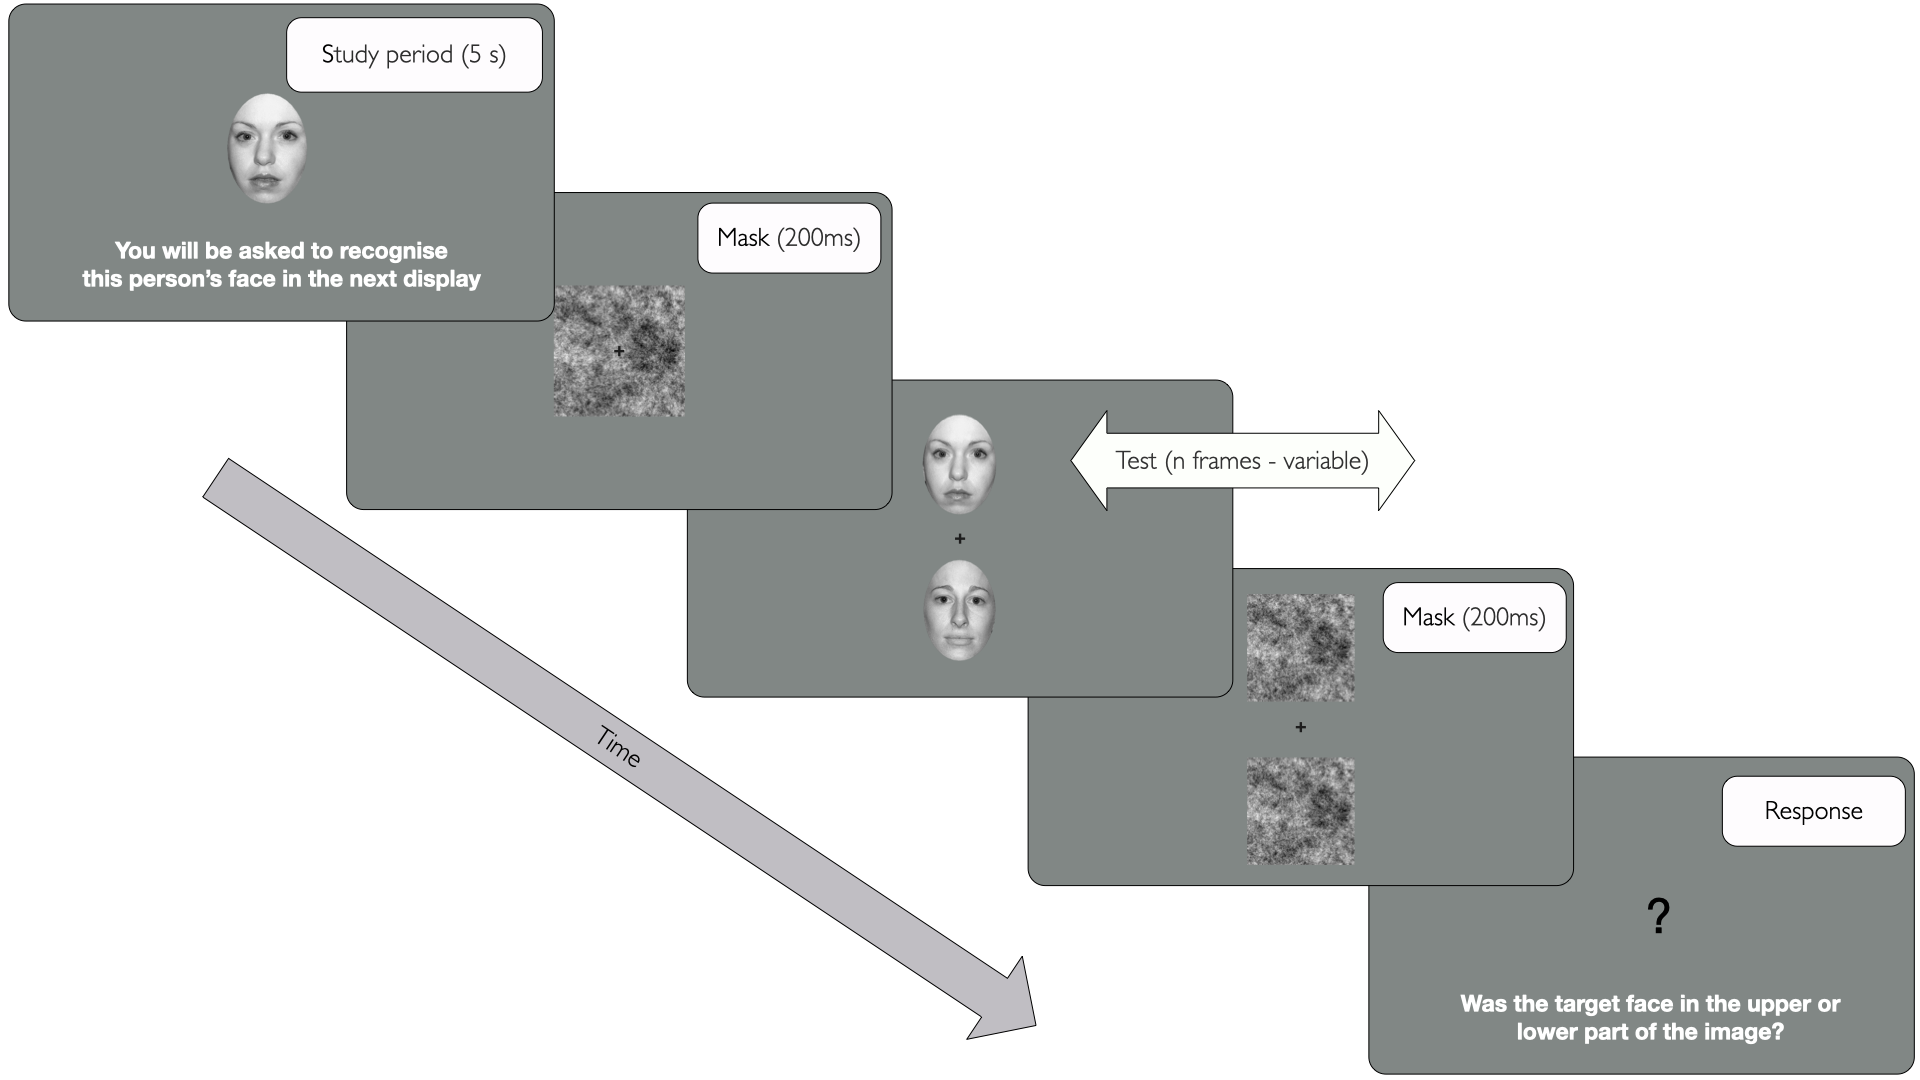
\includegraphics{images/FamiliarFace_Procedure.png}

}

\caption{\label{fig-procedure}The visual stimulation sequence for each
trial}

\end{figure}%

\subsection{Threshold Analysis}\label{threshold-analysis}

In this study we used a staircase procedure to measure face recognition
speed. The staircase began with an easily detected visual display of a
target face and distractor face (see Fig~\ref{fig-procedure}), with the
participant's task being to indicate whether the target face was in the
upper or lower part of the display. Subsequent face stimuli display
times were reduced until the participant made an error, at which point
the staircase reversed so that face stimuli were displayed for longer
periods of time until the participant responded correctly, triggering
another reversal. Image display times were measured in units of 8.33
millisecond video frames. The staircase used a 1-up-3-down design, where
a correct response 3 times in a row generated a reduction in display
time by 1 frame. If the participant made an incorrect response, stimulus
display times increased by 1 frame. Each condition (unfamiliar,
familiar, self-face) included four trials (two with upright faces and
two with inverted faces) and each trial included two randomly
interleaved staircases. The means of the thresholds for each staircase
were averaged to calculate the shortest timeframe in which the face
stimuli could be accurately recognised for each condition.

\subsection{Procedure}\label{procedure}

Participants were verbally briefed on the aim of the research (See
Appendix E) and provided with an information sheet (See Appendix F). An
overview of the task was described as involving recognition of 12 target
faces in a series of displays over the course of the experiment.
Participants were seated opposite a desk with the VIEWPixx display
screen and a keyboard to complete a practice trial to familiarise
themselves with the task (see Fig~\ref{fig-setup}). The practice trial
featured a randomly selected face from the unfamiliar face set, which
was then excluded from the main experiment. A random selection of target
and distractor faces were chosen for each participant. Before each
trial, written instructions appeared on the screen advising participants
to focus on a fixation cross at the centre of the screen and use the up
and down arrow keys to indicate whether the target face appeared above
(up arrow) or below (down arrow) the fixation cross. Participants
pressed any key to continue to initiate the display of a `target' face
stimulus for five seconds. After the inspection period, participants
pressed any key to start the trial. Trials began with a mask stream
followed by a display containing the target face and a distractor face
above and below the fixation cross. The target face appeared randomly
either above or below the fixation cross. Faces were displayed in either
an upright or inverted position.

\begin{figure}

\centering{

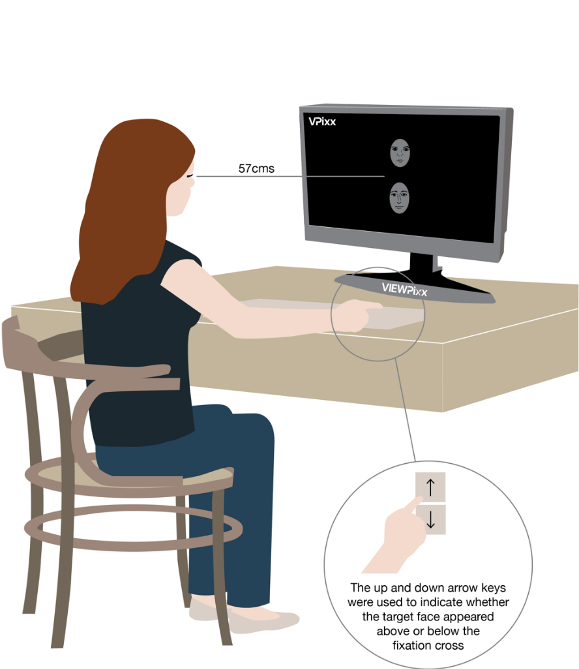
\includegraphics{images/setup.png}

}

\caption{\label{fig-setup}Depiction of experimental setup; image created
by Simone Hale (2023)}

\end{figure}%

\section{Results}\label{results}

\subsection{Data Preparation}\label{data-preparation}

Data analyses were conducted using jamovi (version 2.3.21.0), with
significance levels set to \(\alpha = .05\) for analysis and
\(\alpha = .001\) for assumption testing. Data were examined for missing
responses and no missingness was found. Two participants were excluded
because their threshold scores were consistently above the starting
point of the staircases (18 frames/ 66.67ms) for most of their trials.
Thus, 28 of the original 30 participants were included in the analyses.
Recognition time was measured using the number of frames required to
complete the task as determined by the staircase procedure. Frames were
then converted to milliseconds based on the monitor refresh rate of 120
Hz. Reaction time was measured in milliseconds.

\subsection{Data Analysis}\label{data-analysis}

Assumption testing for the two-way repeated-measures analysis of
variance (ANOVA) indicated no violated assumptions. Visual inspection of
Q-Q plots showed a normal distribution of face recognition times in each
condition and no obvious outliers. Homogeneity of variance was assumed,
as Fmax scores were below 10, in both upright, \(F_{max} = 2.110\), and
inverted, \(F_{max} = 1.697\), orientations. Mauchly's test indicated
that the assumption of sphericity was not violated for the main effect
of condition, \(W(28) = 0.82, p = .081\) and the interaction between
condition and face orientation, \(W(28) = 0.93, p = .399\).

A 2 x 3 repeated-measures analysis of variance (ANOVA) was used to
explore the effects of face familiarity on face recognition time. The
ANOVA showed a main effect of familiarity, with significant differences
in face recognition times between unfamiliar, familiar and self-face
conditions \(F(2, 52) = 48.08, p < .001, \eta_p^2 = .649\). In support
of the first hypothesis, post hoc comparisons with Bonferroni
corrections showed participants recognised their own faces at shorter
display times compared with less familiar faces,
\(t(26) = 3.99, p = .001\), and unfamiliar faces,
\(t(26) = 11.12, p < .001\). The second hypothesis was also supported,
as a post hoc comparison showed participants recognised the familiar
face (that of the experimenter) at shorter display times than unfamiliar
faces, \(t(26) = 5.11, p < .001\).

Results also supported the third hypothesis that participants would
require longer display times to recognise all faces when displays were
inverted. The ANOVA indicated a main effect of orientation for face
recognition times, \(F(1, 26) = 50.22, p <.001, \eta_p^2 = .659\). In
addition, the fourth hypothesis was supported: the face inversion effect
was reduced for more familiar faces. The ANOVA indicated a significant
interaction between condition and face orientation,
\(F(2, 52) = 11.21, p < .001, \eta_p^2 = .301\). The effects of
inversion on recognition time were reduced when faces were more
familiar. Fig~\ref{fig-recognition-times} shows recognition times for
inverted and upright face orientations for each condition.

\phantomsection\label{cell-fig-recognition-times}
\begin{figure}[H]

\centering{

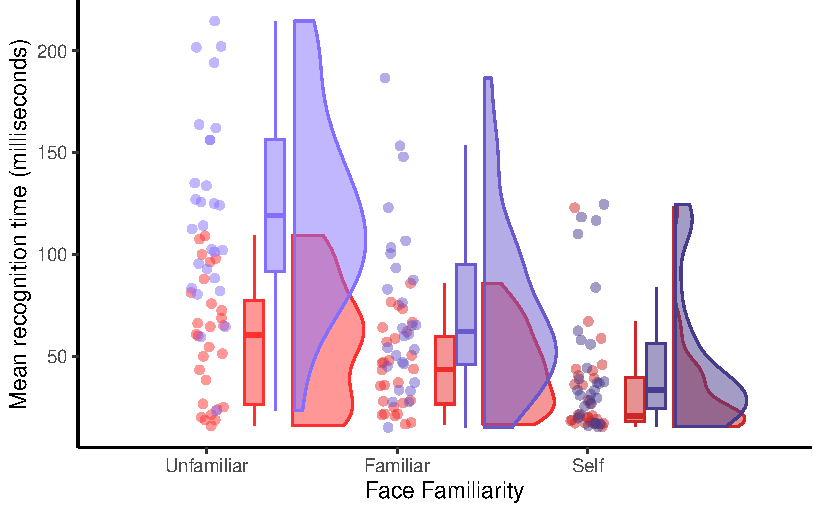
\includegraphics{index_files/figure-pdf/fig-recognition-times-1.pdf}

}

\caption{\label{fig-recognition-times}Recognition Times by Orientation
for Each Condition}

\end{figure}%

\textsubscript{Source:
\href{https://deborahapthorp.github.io/SelfFaceManuscript/index-preview.html}{Article
Notebook}}

A small but significant interaction was also observed between age and
condition, \(F(2, 52) = 4.16, p = .021, \eta_p^2 = .138\). For older
participants, longer display times were required to recognise unfamiliar
and familiar faces than younger participants, whereas older participants
required relatively shorter display times to recognise the self-face
compared to younger participants. Fig~\ref{fig-correlations} shows this
interaction in more detail, illustrating the relationship between age
and recognition time in each condition.

\phantomsection\label{cell-fig-correlations}
\begin{figure}[H]

\centering{

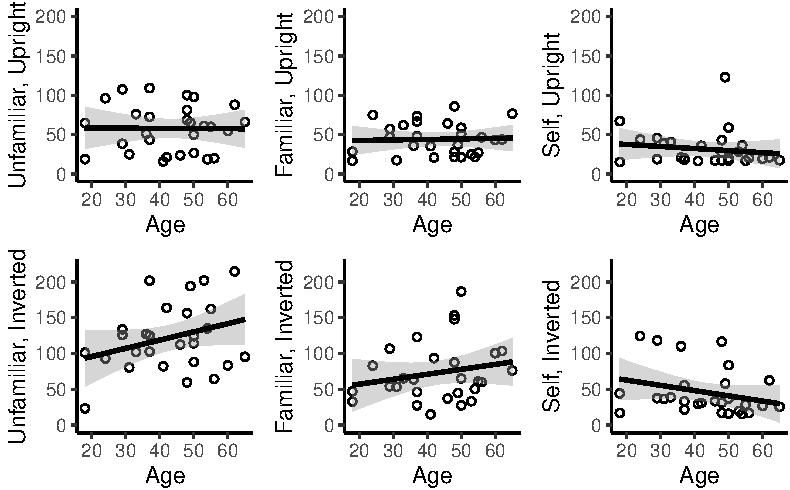
\includegraphics{index_files/figure-pdf/fig-correlations-1.pdf}

}

\caption{\label{fig-correlations}Correlations between recognition times
by age for each condition}

\end{figure}%

\textsubscript{Source:
\href{https://deborahapthorp.github.io/SelfFaceManuscript/index-preview.html}{Article
Notebook}}

\subsection{Exploratory Analysis}\label{exploratory-analysis}

\subsubsection{Reaction Time}\label{reaction-time}

An identical 2 x 3 repeated measures ANOVA was conducted on participant
reaction times (computed as the elapsed time between stimulus
presentation and button press), to identify whether reaction times would
also reveal a familiarity effect in face recognition. The ANOVA showed a
main effect of face condition, with faster reaction times for the more
familiar faces, \(F(2, 52) = 3.85, p = .028, \eta_p^2 = .129\). There
was also a significant main effect of face orientation, with longer
reaction times for inverted faces,
\(F(1, 26) = 18.71, p <.001, eta_p^2 = .418\). However, there was no
significant interaction between condition and face orientation,
\(F(2, 52) = 0.14, p = .872, eta_p^2) = .005\).
Fig~\ref{fig-reaction-times} shows reaction times for inverted and
upright face orientations for each condition.

\phantomsection\label{cell-fig-reaction-times}
\begin{figure}[H]

\centering{

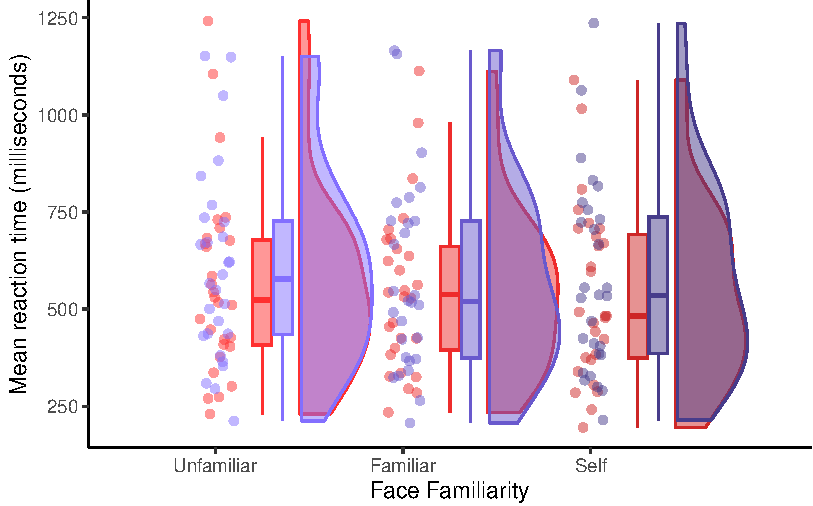
\includegraphics{index_files/figure-pdf/fig-reaction-times-1.pdf}

}

\caption{\label{fig-reaction-times}Reaction times by orientation for
each condition}

\end{figure}%

\textsubscript{Source:
\href{https://deborahapthorp.github.io/SelfFaceManuscript/index-preview.html}{Article
Notebook}}

\section{Discussion}\label{discussion}

To better understand the effect of greater levels of familiarity on face
recognition, the present study used a staircase procedure to
characterise face recognition performance. Participants responded to
three different face categories manipulated by familiarity (unfamiliar,
familiar, and self), and orientation (upright and inverted). Recognition
time (i.e., perceptual processes) was isolated from reaction time (i.e.,
perceptual processes + cognitive decision + motor response) and used as
an index of the familiarity effect. The overall findings confirmed
predictions that more familiar faces are processed faster than less
familiar and unfamiliar faces. Notably, our results underscore the
self-face as a unique class of familiar face, providing compelling
evidence for distinct perceptual processing.

\subsection{Familiarity and Recognition
Time}\label{familiarity-and-recognition-time}

In support of hypothesis one, participants recognised their own faces at
shorter display times compared with other faces, providing evidence for
distinct perceptual processing \citep{alzueta2019a, rooney2012a}.
Results conflicted with an EEG study demonstrating the self-face
elicited similar neural responses relative to personally familiar faces
\citep{wiese2021a}. The self-face advantage observed in the recognition
times may reflect robust self-representations developed over time,
strengthened by both the amount of exposure and the nature of the
exposure we have with our own face \citep{bortolon2017a, tong1999a}. For
example, examining our image in the mirror is a multisensory encounter,
allowing us access to motor-sensory and tactile cues that enable us to
update our mental representations of ourselves \citep{bortolon2017a}.
Further, research linking self-face recognition and self-esteem revealed
that when participants viewed photographs of themselves alongside images
that were manipulated to look more attractive, observers chose the
manipulated images as more accurate self-representations, which
correlated with higher self-esteem \citep{felisberti2014a}. This
tolerance to error, as reflected by the perceptual biases, may be a
crucial and distinctive component of self-face representations that
could enhance recognition performance \citep{felisberti2014a}.

Familiarity effects were also found in the shorter display times
required to recognise the familiar face (the experimenter) compared to
unfamiliar faces, supporting hypothesis two. The findings align with the
abundant research evidence in face recognition demonstrating a
qualitative and quantitative gap between familiar and unfamiliar face
processing \citep{burton2013a, burton2016a, ramon2017a}. It is possible
that familiar face recognition performance was strengthened by the
opportunity for participants to learn how the experimenter's face
changed in appearance (e.g., different facial expressions and viewing
angles), and the conceptual information (name and research interest)
shared prior to the experiment \citep{dowsett2016a}.

The observation that older participants were faster at recognising their
own face compared to younger participants was surprising given the rise
in the importance of the ``selfie'' in youth culture
\citep{tshidzumba2019a}. In line with previous research suggesting that
we are better at discriminating faces from our own age group, it is
possible that older participants found it easier to distinguish their
own face from the distractor faces, which were young identities (See
Appendix C; \citet{rhodes2012a}).

\subsection{Familiarity and Inversion
Effects}\label{familiarity-and-inversion-effects}

The present study replicated the face inversion effect, a common finding
in previous research that suggests human participants experience more
difficulty recognising faces when they are upside down than when they
are upright in their canonical orientation. Therefore, these findings
support the third hypothesis, that regardless of familiarity, faces are
harder to recognise upside down
\citep{allen-davidian2021a, kramer2018a, taubert2011a, young2017a}. This
experiment also yielded empirical support for hypothesis four; the face
inversion effect was significantly smaller for familiar faces than
unfamiliar faces. Interestingly, the more familiar participants were
with the face, the more immune they were to the inversion manipulation.
This finding is consistent with previous studies that have also
suggested that familiar faces are robust to the deleterious effects of
inversion \citep{keyes2012a, keyes2010a, yang2014a}. However, results
contradicted those of \citet{alzueta2019a}, who found no significant
change in the size of inversion effects across unfamiliar, familiar and
self-face conditions. Inconsistent findings may be explained by the
difference in task complexity between the studies. For example, the
staircase used in the present study involved finding a target face
between two images, displayed for a short period (e.g., 66.67ms starting
point), averaging performance across 12 trials, whereas
\citet{alzueta2019a} allowed participants 1000ms to categorise a single
face display as ``me'', ``friend'' or ``stranger'', averaging
performance across 450 trials.

Overall, these findings provide strong behavioural support for the idea
that images of our face are processed differently to other faces, as
participants were able to easily recognise their own face in the
inverted position in less time than was required to recognise an upright
unfamiliar face. The current results challenge the widely accepted view
that all human faces are processed holistically, as the faster
recognition times for inverted faces in the familiar and self-face
conditions could be interpreted as evidence for stronger feature-based
representations \citep{gerlach2022a, tong1999a}.

\subsection{Reaction Time and Levels of
Familiarity}\label{reaction-time-and-levels-of-familiarity}

Consistent with recognition time results and in alignment with the
literature, there was a significant difference in reaction times between
unfamiliar, familiar and self-face conditions
\citep{kloth2006a, ramon2011a, young2017a}. Interestingly, the reaction
times were found to be longer than those reported in other studies,
which is likely due to the inherent task complexity when using a
staircase, compared to more simple, untimed go/no-go face categorisation
tasks \citep{bortolon2017a, burton2016a, ramon2011a, smith2016a}.

Importantly, the data revealed that recognition times were substantially
shorter than reaction times for each condition. For example, on average,
participants recognised (processed) upright familiar faces within 43.8ms
but required 547ms to respond (process + decision + motor response) to
the target face. These findings have important implications for future
research designs, as they suggest that reaction times may be
underestimating face recognition performance. Reaction times were longer
for inverted faces compared to upright faces, however, the data did not
reveal the interaction observed in the recognition time data, as there
was no significant difference in the face inversion effect between
conditions. Thus, recognition time seems to be a more sensitive measure
of familiarity effects in face recognition.

\subsection{Limitations and Future
Directions}\label{limitations-and-future-directions}

The staircase procedure was a key strength of the research,
demonstrating that the reaction times reported in research may be
underestimating human face recognition ability
\citep{besson2016a, caharel2014a, ramon2011a}. However, the study design
represented some limitations centred around comparability with other
face recognition research. First, recognition times cannot be directly
compared with reaction times. Second, the staircase procedure only
measured the ability of participants to discriminate between two
stimuli, unlike other studies that require participants to identify a
target face among an array of distractor faces \citep{megraya2006a}.
Third, the time constraint imposed by the staircase is not comparable
with studies involving tasks without time limits
\citep{zimmermann2019a}. Future studies could attempt to address some of
these comparability concerns by replicating the same study together with
a standard go/no-go face categorisation task, to allow for a comparison
of reaction times between the two tasks. Further, adapting the staircase
to include a four alternative force choice task, compared to the two
alternatives used here, would provide a better comparison with studies
involving recognition tasks that require discrimination between multiple
exemplars. Although the study examined three levels of familiarity
(unfamiliar, familiar, and self), other highly familiar faces such as
famous faces were not included \citep{campbell2020a, wiese2021a}. Future
studies could incorporate famous faces and face stimuli of identities
that are more intimately known by the perceiver such as close friends
and family members, to test the effects of different levels of
familiarity on face recognition in both upright and inverted
orientations. This would allow further exploration of the inversion
effect found in the present study. It would also assist future face
recognition research in defining the familiarity construct, particularly
with respect to the self-face compared with other highly familiar faces.
Further, the varying levels of familiarity participants had with the
experimenter created inconsistency in the construct of the familiar
condition. Future studies could include a larger sample of both
previously unknown and previously known participants to compare the
performance of two different levels of familiarity. Including previously
unknown participants also provides valuable insight into the effects of
real-world face learning on recognition.

Future research should aim to involve diverse participants, including
males and representation from all age groups. The female only sample may
have influenced results, as there is some evidence suggesting a female
own-gender bias in face recognition performance
\citep{herlitz2013a, lov2011a, mishra2019a}. The mean age (43.1 years)
in the present study is not reflective of the average age
(\textasciitilde{} 21-35 years) of participants in many other face
recognition studies
\citep{kloth2006a, mohr2018a, pachai2017a, platek2009a}. Including a
range of age groups is warranted given the age interaction found in the
present study and research suggesting an age-bias in face recognition
performance \citep{rhodes2012a}.

\subsection{Conclusion}\label{conclusion}

Overall, the findings of the present study demonstrate the familiarity
advantage in face recognition. We provide strong evidence in support of
distinct perceptual processing at different levels of familiarity, as
demonstrated by faster recognition times for both the self-face and
familiar face compared to unfamiliar faces. The self-face appears to be
processed differently to other familiar faces, validating the self-face
as an important inclusion in face studies seeking to understand the
familiarity effect in face recognition. The staircase procedure provided
a unique insight into processing time, highlighting the potential
underestimation of face recognition ability in the literature. The
finding that face inversion is less disruptive to the processing of more
familiar faces is further evidence of distinct perceptual processes and
challenges the widely held view that faces are processed holistically.
We recommend further exploration of the effects of inversion at
different levels of familiarity, to enhance understanding of perceptual
processing distinctions, and identify implications for holistic and
featural processing theories.


\nolinenumbers
  \bibliography{selffaces.bib}

\end{document}
